\chapter{Network Internals}\label{ch:07-net-impl}

\section{Command Line Tools}

Before we move on to implementation details,
  let us look at some command line tools.
Our goal is not to become adept at network administration.
Rather, we'll use these tools to start peeking under the hood,
  at the implementation of TCP/IP\null.

Let's see what is the IP address of Google.
{\footnotesize
\begin{verbatim}
  rg@rg-2016:notes$ host www.google.com
  www.google.com has address 216.58.206.36
  www.google.com has IPv6 address 2a00:1450:4009:812::2004
\end{verbatim}
}\noindent
Using the \df{name} \.{www.google.com},
  which is easy to remember,
  we found out that
    (a)~\.{216.58.206.36} is an IPv4 address of Google, and
    (b)~\.{2a00:1450:4009:812::2004} is an IPv6 address of Google.
Note that the IPv4 address is a 32~bit number,
  and the IPv6 address is a 128~bit number.
By convention,
  IPv4 is split into 4~groups which are written in decimal,
  and IPv6 is written in hexadecimal using some more complicated convention.
We could check what is the RTT (round-trip time) using \.{ping},
  as we did in the previous lecture.
Instead, let us extract more information using \.{traceroute}.
{\footnotesize
\begin{verbatim}
  rg@rg-2016:notes$ traceroute -q 1 216.58.206.36
  traceroute to 216.58.206.36 (216.58.206.36), 30 hops max, 60 byte packets
   1  core-196.kent.ac.uk (129.12.196.1)  2.907 ms
   2  fw-cdc-core.kent.ac.uk (129.12.254.25)  3.125 ms
   3  uok-c-pc-10.kentman.ac.uk (212.219.171.129)  3.896 ms
   4  10.49.3.205 (10.49.3.205)  3.871 ms
   5  ic-wye-ge-2-5.kentman.ac.uk (212.219.171.137)  3.476 ms
   6  ae0.londtw-sbr2.ja.net (146.97.41.85)  7.323 ms
   7  ae29.londtn-sbr1.ja.net (146.97.33.10)  7.665 ms
   8  72.14.205.74 (72.14.205.74)  8.023 ms
   9  108.170.246.193 (108.170.246.193)  9.193 ms
  10  216.239.41.207 (216.239.41.207)  8.823 ms
  11  lhr35s10-in-f4.1e100.net (216.58.206.36)  9.178 ms
\end{verbatim}
}\noindent
Is there any open socket currently?
{\footnotesize
\begin{verbatim}
  rg@rg-2016:notes$ ss -t
  State      Recv-Q Send-Q Local Address:Port                 Peer Address:Port                
  ESTAB      0      0      129.12.196.69:53204                74.125.133.188:5228  
\end{verbatim}
}\noindent
Running \.{whois 74.125.133.188} we can check that the peer
  is (another IP address of) Google.
But, the output of \.{whois} is quite verbose.
Incidentally, \.{host} does not only name lookups but also reverse lookups:
{\footnotesize
\begin{verbatim}
  rg@rg-2016:notes$ host 74.125.133.188
  188.133.125.74.in-addr.arpa domain name pointer wo-in-f188.1e100.net.
\end{verbatim}
}\noindent
Alas, the name \.{wo-in-f188.1e100.net} is neither suggestive,
  nor easy to remember.

Earlier, when I said \.{traceroute 216.58.206.36},
  how did the computer choose the next hop,
    which was \.{129.12.196.1}?
For that, I need to look at the routing table:
{\footnotesize
\begin{verbatim}
  rg@rg-2016:notes$ ip route
  default via 129.12.196.1 dev wlan0  proto static  metric 600 
  10.0.3.0/24 dev lxcbr0  proto kernel  scope link  src 10.0.3.1 linkdown 
  129.12.196.0/22 dev wlan0  proto kernel  scope link  src 129.12.196.69  metric 600 
  169.254.0.0/16 dev docker0  scope link  metric 1000 linkdown 
  172.17.0.0/16 dev docker0  proto kernel  scope link  src 172.17.0.1 linkdown 
  192.168.240.240 via 129.12.196.1 dev wlan0  proto dhcp  metric 600
\end{verbatim}
}%
All entries start with a pattern, and then continue with instructions.
The pattern \.{default} applies when no other pattern does.
A pattern like \.{10.0.3.0/24} is called a \.{mask},
  and it matches a set of destination addresses,
  namely those that start with the same 24~bits as \.{10.0.3.0}.
We can check that our destination address (\.{216.58.206.36})
  does not match any pattern in the routing table,
  so the default rule applies.
The default rule says
  what the next hop should be (\.{via 129.12.196.1}),
  which physical device should be used (\.{dev wlan0}),
  and also gives a cost to using this rule (\.{metric 600}).

But, can we send packets to \.{129.12.196.1} directly?
That is, is it our neighbour?
{\footnotesize
\begin{verbatim}
  rg@rg-2016:notes$ ip neighbor
  129.12.196.1 dev wlan0 lladdr 00:08:e3:ff:fc:50 REACHABLE
\end{verbatim}
}\noindent
Oh: it is our only neighbour.
Also, we find out that its physical address is \.{00:08:e3:ff:fc:50}.
Typing this in at \url{https://macvendors.com/},
  we find out that the network card of our neighbour was manufactured by Cisco.
What about our network card?
{\footnotesize
\begin{verbatim}
  rg@rg-2016:notes$ ip link show dev wlan0
  3: wlan0: <BROADCAST,MULTICAST,UP,LOWER_UP> mtu 1500 qdisc mq state UP mode DORMANT group default qlen 1000
      link/ether 18:5e:0f:e0:bb:72 brd ff:ff:ff:ff:ff:ff
\end{verbatim}
}\noindent
Using \.{18:5e:0f\dots} we can check that the manufacturer is Intel.
Why is it possible to do this?
Because physical addresses were originally meant to be globally unique,
  and there was a mechanism put in place to allocate
    which range of addresses a manufacturer is allowed to use.
(By the way, \.{lladdr} stands for `link-layer address',
  which means the same as `physical address',
  but emphasizes which layer uses the address.)
That was the original plan, however.
Nowadays, most hardware makes it easy to change the physical address.
Technically,
  link-layer addresses only need to be unique among the computers
  that are physically connected.
Plus, IPv6 has way more addresses than the link-layer does.
So, it makes less and less sense to insist on globally unique link-layer addresses.


\section{Network Protocols: IP, OSPF, IS-IS, BGP}

Now that we've poked at the surface, let us dive into some internals.
The main protocol implemented in the network layer is IP\null.
The main task of IP is to deliver packages to their destination.
IP packets have a payload, which is prefixed by a header.
The format of the header is as follows:
\begin{center}
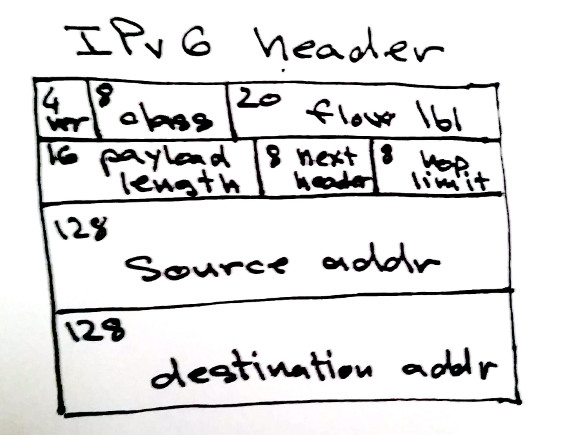
\includegraphics[width=.5\textwidth]{ipv6-header.jpg}
\end{center}
\todo{tikz}
The real layout is, of course, one dimensional:
  we pack fields in a two dimensional drawing
    because it lets us easily see the whole headers,
    without moving our eyes much.
The most important field here is the \emph{destination address}.
Without a destination address,
  IP could not carry out its job of delivering packets towards their destination.
The typical job of an IP router is as follows:
  (1)~look at the destination address,
  (2)~see which pattern in the routing table it matches, and
  (3)~execute the instructions found in the matching routing table entry.
Next in importance comes the \emph{source address}.
After all, Internet is built for conversations not for lectures.
To reply to a message, you need to know who sent it.
Both addresses, for the destination and for the source, are groups of 128~bits,
  because we are looking at IPv6.

The \emph{version} field allows one to migrate from one version to another.
IPv4 and IPv6 can coexist in the same network
  because we can easily tell apart the packets of one from the packets of the other,
  by looking at the first few bits.
This trick, of including a version number somewhere near the beginning,
  is widely used in data formats.
For example,
  Java bytecode always starts with \.{0xCAFEBABE}
    (so you can easily tell this is a file with Java bytecode),
  followed by 4~bytes that give the version.

The \emph{payload length} field counts bytes.
Since there are 16~bits for this field,
  the payload of an IPv6 packet can be at most $2^{16}$~bytes.
Or so it seems:
  there is a way to get around this limitation,
  but we will not discuss it because it isn't used often.
The \emph{next header} field has a few predefined values
  that indicate what type of payload is carried.
The most common values indicate TCP and UDP\null.

The \emph{hop limit} is an integer that gets decremented by every router.
When this counter reaches~0,
  routers throw the packet away,
  instead of routing it.
This mechanism ensures that packets cannot travel forever in a network,
  which otherwise might happen if routing tables would contain incorrect information.

The \emph{class} and \emph{flow label} fields are sometimes used for advance features,
  which we will not discuss.
But, roughly,
  the class could indicate whether this packet cares
    more about bandwidth or more about latency;
  while the flow label could be used to make
      it easy to identify all packets used for a particular video-chat conversation.
Note that such features (bandwidth-vs-latency, chat-vs-download)
  are typically considerations for the application layer.
But, it can clearly help if the routing is done in a way
  that is application-aware.

\medskip

The next question is this: where do routing tables come from?
One option is for a system administrator to configure them,
  using a tool such as `\.{ip route}'.
But, recall the initial motivation for designing the Internet:
  to have a network that reconfigures itself when parts of it are destroyed.
If we require humans to decide which routes packets take,
  then such reconfiguration would be slow.
Instead, there exist a number of routing protocols,
  such as OSPF, IS-IS, and BGP,
  whose purpose is to build routing tables.

What is the difference between these protocols?
OSPF and IS-IS are \emph{intra}-domain routing protocols;
  BGP is an \emph{inter}-domain routing protocol.
Very roughly,
  a domain (aka {\bf a}utonomous {\bf s}ystem)
  is a big chunk of the Internet that has one owner.
The technical differences between OSPF and IS-IS are rather subtle.
But, while OSPF is \emph{open},
  most ISPs ({\bf I}nternet {\bf s}ervice {\bf p}roviders) prefer IS-IS\null.

The difference between inter- and intra- domain protocols is less subtle:
  inter-domain protocols allow humans much more control
    over how routes are chosen.
The traffic that flows from one domain to another
  is often subject to a commercial contract:
  one cannot simply let computers chose the best path when money is involved.
But, perhaps more importantly,
  fully automatic protocols do not scale to the whole of the Internet.
The restrictions put in place by humans to honour commercial contracts
  are in fact helpful for reducing the search space for routing algorithms.

BGP allows sysadmins to provide high-level (mostly declarative) rules
  that guide the process of building routing tables.
One open area of research nowadays
  is to develop tools that analyse these high-level rules to see whether
  they could possibly lead to bad situations, such as network partitions.


\section{Routing Algorithms}

Most routing algorithms are based on the simple observation
  that a shortest path has a first step.
Suppose we want to find the shortest path from some source~$s$ to some target~$t$.
Then, $s$~could ask one of its neighbours, let's call it~$n$,
  what is the shortest path from~$n$ to~$t$.
If $n$~answers, then $s$ knows one candidate shortest path:
  go to $n$, and then let $n$ do the rest.
There is, of course, one such candidate solution for each neighbour~$n$.
If $s$~asks around all its neighbourhood,
  then it must be that the shortest path is one of the candidates considered.
In other words, the following holds:
\begin{align}
d(s,t) =
  \begin{cases}
  0 &\text{if $s=t$} \\
  \min_{n \in N(s)} \bigl(c(s,n) + d(n,t)\bigr) &\text{if $s\ne t$}
  \end{cases}
\label{eq:dist}
\end{align}
Here,
\begin{itemize}
\item $d(x,y)$~is the distance from~$x$ to~$y$,
\item $c(x,y)$~is the cost of the direct link from~$x$ to~$y$, and
\item $N(x)$~is the neighbourhood of~$x$;
  that is, $N(x) \defeq \{\,y\mid c(x,y)<\infty \,\}$.
\end{itemize}
In words,
  the distance form a source~$s$ to a target~$t$ corresponds
    to making a first step from~$s$ to some neighbour~$n$,
  and then continuing on a shortest path from~$n$ to~$t$.
We assume that initially we know the costs $c(x,y)$
  for all network interfaces $x$~and~$y$;
  we require
\begin{align}
  c(x,y) &= \infty &&\text{if there is no direct link from~$x$ to~$y$}
\\
  c(x,x) &= 0 &&\text{for all $x$}
\end{align}
The distances $d(x,y)$, however, are unknown.
Imagine, for now, that we have a big 2-dimensional matrix~$D$,
  and we'll set things up such that
\begin{align}
  D[x][y] &\ge d(x,y)
  &&\text{for all $x$~and~$y$}
  \label{eq:dub-1}
\intertext{and}
  D[x][z] &\ge \min_{y\in N(x)} \bigl(c(x,y) + D[y][z]\bigr)
  &&\text{for all $x$~and~$z$}
  \label{eq:dub-2}
\end{align}
Think of costs~$c$ and distances~$d$ as immutable --- they don't change.
The matrix~$D$, however, is changing:
  it is an approximation of the distances~$d$,
  which will be a really bad approximation in the beginning,
    but it will get better and better.

In the beginning,
  we set $D[x][y] \asgn \infty$ for all $x \ne y$,
  and $D[x][x] \asgn 0$ for all~$x$.
Note that, now, both \eqref{eq:dub-1}~and~\eqref{eq:dub-2} hold trivially;
  that is, they hold because of how we set up $D$,
    irrespective of the costs and distances.
Our goal is to decrease the values in the matrix~$D$
  so they get closer and closer to the distances~$d$.
While doing this,
  we will be careful to keep \eqref{eq:dub-1}~and~\eqref{eq:dub-2} true.
What we'll do is to repeatedly apply an operation called \df{relaxation},
  until it is not possible to apply any more.
It is possible to apply a relaxation as long as we find $s$, $n$, and~$t$
  such that
\begin{align}
  D[s][t] > c(s,n) + D[n][t]
\end{align}
A relaxation consists in doing the update
\begin{align}
  D[s][t] \asgn c(s,n) + D[n][t]
\end{align}
Clearly, \eqref{eq:dub-2} still holds for $x\asgn s$ and $z\asgn t$.
Instantiations of~\eqref{eq:dub-2} for other values of $x$~and~$z$ are also OK
  because $D[s][t]$ can only be on their right hand side (and it decreased).
Did we break \eqref{eq:dub-1} for $x\asgn s$ and $y \asgn t$?
No, because
\begin{align*}
D[s][t]
  &\ge \min_{n\in N(s)} \bigl(c(s,n)+D[n][t]\bigr)
    &&\text{by \eqref{eq:dub-2}}
\\
  &\ge \min_{n\in N(s)} \bigl(c(s,n)+d(n,t)\bigr)
    &&\text{by \eqref{eq:dub-1}, with $x\ne s$}
\\
  &= d(s,t)
    &&\text{by \eqref{eq:dist}}
\end{align*}
So, if \eqref{eq:dub-1}~and~\eqref{eq:dub-2} were true before relaxing,
  they are still true after relaxing.
We say that relaxation \emph{maintains} \eqref{eq:dub-1}~and~\eqref{eq:dub-2}.
When a relaxation is not possible any more, it means that
\begin{align}
  D[s][t] &\le c(s,n) + D[n][t]
  &&\text{for all $s,n,t$}
\end{align}
From this and \eqref{eq:dub-2},
  it follows that $D$ satisfies~\eqref{eq:dist},
  which is essentially our definition of what a distance is.

There exist several algorithms, such as Dijkstra and Bellman--Ford,
  which differ in the order they perform relaxations.
We won't care much about the order,
  since pretty much any order works.
(True, some work faster.)

\medskip

For routing in networks, we could
\begin{enumerate}
\item implement the sketch above in a distributed way, or
\item make sure each computer knows the structure of the whole network,
  and runs the above algorithm on its own (so, not distributed).
\end{enumerate}
The first solution was used until $\sim1979$;
  the second solution is used nowadays
    because it reacts faster to changes in the network topology.
Let's discuss them in turn.

In the distributed setting, $D[x]$ is stored at~$x$.
Suppose that $D[x][y]$ is the distance from~$x$ to~$y$, as discussed above.
Let us now see what happens when the network changes:
  $c(x,y)$ decreases or increases.
Perhaps the link goes down, or becomes faster, or is a new link.
Before, we have not considered changes of the cost~$c$,
  so we are now looking at a new phenomenon.
When $c(x,y)$ changes, we assume that $x$~notices it somehow.
When that happens, it runs the update $D[x][y] \asgn c(x,y)$,
  with the \emph{new} cost~$c(x,y)$.
Another rule is that each node informs its neighbours whenever it updates
  an entry of~$D$.
If $x$~updates $D[x][y]$,
  then it will send a message to each neighbour,
  telling it what is the new value of $D[x][y]$.
In summary, each node~$x$ follows two simple rules:
\begin{itemize}
\item if $c(x,y)$ changes, then update $D[x][y] \asgn c(x,y)$, and
\item if $D[x][y]$ changes, then inform all neighbours of the change.
\end{itemize}
Of course, when a node~$z$ finds out that $D[x][y]$ changed,
  it will consider whether it can update $D[z][y]$ via a relaxation.
And, if it does, then it will in turn inform its neighbours
  of the change in $D[z][y]$.
And so on, the updates propagate.

If a new node joins the network, or if a node leaves the network,
  then this is the same as updating several costs~$c$;
  namely, those costs involving the interesting node.

The distributed algorithm sketched so far has a correctness issue.
Our argument for correctness relied on costs not changing and on several invariants;
  in particular, we are supposed to have $D[x][y] \ge d(x,y)$.
It turns out that we can extend our correctness argument for situations
  in which costs $c(x,y)$ may \emph{decrease}.
However,
  if costs may increase, as it happens if a link or a node fail,
  then the algorithm sketched above is in fact incorrect.
Intuitively,
  the issue is that the algorithm does not propagate information
  about costs that become worse (that is, larger).
Thus, nodes that are not immediately next to the modified link
  will think that it is still possible to use the previous (now unavailable) cost.
Formally,
  increasing the cost~$c$ will increase distances~$d$
  which in turn breaks our invariant $D[x][y] \ge d(x,y)$,
  and that breaks our correctness argument.

\begin{figure}
\begin{alg}
\^  on a change of $c(x,y)$
\0 $D[x][y] \asgn c(x,y)$
\end{alg}
\smallskip
\begin{alg}
\^  on receiving $y \to x : (z, \alpha)$
\0  $\delta \asgn c(x,y) + \alpha$
\0  if $N[x][z]=y$
\1    $D[x][z] \asgn \delta$
\0  else if $D[x][z] > \delta$
\1    $D[x][z] \asgn \delta$
\1    $N[x][z] \asgn y$
\end{alg}
\smallskip
\begin{alg}
\^  on a change of $D[x][y]$
\0  for each $z \in N(x)\setminus\{x,y\}$
\1    send $x \to z : (y, D[x][y])$
\end{alg}
\smallskip
\begin{alg}
\^  every once in a while, for random $x,y,z$
\0  send $x \to y : (z, D[x][z])$
\end{alg}
\caption{
  Distributed routing algorithm.
  The notation $y \to x : (z, \alpha)$ stands for a message from~$y$ to~$x$
    which says that $y$~knows how to reach~$z$ with a cost of~$\alpha$.
  The best guess for the distance from~$x$ to~$y$ is stored in $D[x][y]$;
    and the corresponding next hop is stored in $N[x][y]$.
  Note that $D[x]$~and~$N[x]$ are stored by node~$x$,
    so they can only be read/written by node~$x$.
}
\label{fig:distributed-routing}
\end{figure}

\autoref{fig:distributed-routing} shows one naive attempt to re-establish correctness.
The main difference from the algorithm sketched above
  is that $D[x][z]$~\emph{may} increase on line~3 of handling a message,
  but only if the message comes from the next hop $N[x][z]$.
The other difference is that distances $D[x][y]$ are broadcast regularly,
  even if they have not changed.
The intention is that the following will eventually hold, once the cost stabilizes:
\begin{align}
  D[x][y] &= c\bigl(x,N[x][y]\bigr) + D\bigl[N[x][y]\bigr][y]
    &&\text{for $x\ne y$}
\end{align}
Indeed, suppose that the above does not hold for some $x\ne y$.
\todo{check this a bit more carefully}
Then, eventually, there will be a message $N[x][y] \to x : (y,D[N[x][y]][y])$,
  which will fix the problem.
This argument, however, does not suggest a rapid convergence.

\medskip

To improve the rate of convergence,
  modern routing algorithms, like those of OSPF and IS-IS, are not distributed.
Instead, each node periodically broadcasts what it sees around and,
  at the same time, each node stores structure of the whole network.
\todo{start with some examples}
A node~$x$ will periodically transmit, to all its neighbours,
  a packet that lists all its neighbours~$y$, and the cost $c(x,y)$ of reaching them:
\[
  x, k, \bigl(y_1, c(x,y_1)\bigr), \ldots, \bigl(y_n, c(x,y_n)\bigr)
    \qquad\text{where $\{y_1,\ldots,y_n\}$ is $x$'s neighbourhood}
\]
Here, $k$~is a counter that starts at~$0$
  and is incremented every time $x$~initiates such a broadcast.
These packets need to be forwarded by other nodes.

Each node also maintains an image of the whole network.
It does so by remembering, for each node~$x$, the last broadcast initiated by~$x$.
It knows which broadcast is last not because it arrived last
  but because it has the highest value of the counter~$k$;
  after all, messages can overtake each-other.
The entry associated with node~$x$ also gets a timestamp~$t$
  that records when the broadcast was received.
Thus, the data structure maintained by \emph{each} node looks as follows:
\begin{align}
\begin{array}{cccccc}
  x_1 & k_1 & t_1 & (y_{11}, c_{11}) & (y_{12}, c_{12}) & \ldots \\
  x_2 & k_2 & t_2 & (y_{21}, c_{21}) & (y_{22}, c_{22}) & \ldots \\
  &&\vdots\\
  x_n & k_n & t_n & (y_{n1}, c_{n1}) & (y_{n2}, c_{n2}) & \ldots \\
\end{array}
\label{eq:graph-rep}
\end{align}
If the entry is not refreashed within a certain time,
  by receiving a broadcast with a higher~$k$,
  then node~$x$ is assumed dead, and all knowledge of it is erased.
Note that the data structure from above is not a \emph{square} matrix,
  because different nodes have neighbourhoods of different sizes.

How are broadcasts forwarded?
When a message $(x,k,L)$ is received,
  a node first checks if it has already a line for~$x$
    with a $k$ just as big or bigger.
If so, then nothing is done.
Otherwise, the row for~$x$ is updated,
  and the message is forwarded to all neighbours.

Finally, each node uses the data structure~\eqref{eq:graph-rep}
  to run its own (non-distributed) shortest path alorithm.
The data structure~\eqref{eq:graph-rep} is not guaranteed to be the same at all nodes.
In fact, we can expect that most of the time there exist small discrepancies.
Because of this,
  routing decisions taken by different nodes might be incompatible,
  in the sense that they might lead to anomalous situations,
    such as a packet going round and round in cycles.
But, such anomalous situations should not last for long.
Also,
  note that storing all of~\eqref{eq:graph-rep} for the whole of Internet
    is problematic,
  which is why inter-domain protocols such as BGP are not fully automatic.


\section{Exercises}

\begin{enumerate}
\item
  $\blacktriangleright$
  Here is a list of command line tools that are useful for understanding the network:
  \.{curl},
  \.{dig},
  \.{ip},
  \.{iptables},
  \.{nmap},
  \.{ping},
  \.{ss},
  \.{tc},
  \.{tcpdump},
  \.{traceroute},
  \.{wget},
  \.{whois}.
  Install them, and look at their \.{man} pages.
\item
  $\blacktriangleright$
  To observe network traffic, install and play with \.{wireshark}.
\item
  To see all the network interfaces on your system,
    run `\.{ip link}'.
\item
  To see which servers and on which ports are running on your computer,
    run `\.{nmap 127.0.0.1}'.
  Figure out how to do something similar by using \.{ss}.
\item
  $\blacktriangleright$
  Give a list of four websites that are likely to use UDP\null.
  Connect to them, and check whether they do indeed start UDP connections.
  [Hint: Use \.{ss}.]
\item
  $\blacktriangleright$
  What is the size of an IPv6 header, in bytes?
\item
  For the basic routing algorithm,
    we showed that
      \emph{if} it terminates
      then the matrix~$D$ satisfies the definition~\eqref{eq:dist} of distances.
  But, \emph{does} it terminate?
\item
  The discussion on routing algorithms assumes, for simplicity,
    that each network interface acts independently.
  In reality,
    instead of having a routing table per network interface,
    we have one routing table per computer,
    which may have multiple network interfaces.
  How does this affect our discussion about routing?
\item
  The text gives a correctness argument for algorithms that find shortest paths
    based on a sequence of relaxations.
  Extend the argument for situations in which the costs of links may decrease
    while the argument runs.
\end{enumerate}

\section{Notes}

\begin{itemize}
\item[{[1]}]
  Tanenbaum, Wetherall,
  \emph{Computer Networks}, Chapter~5,
  2011
\item[{[2]}]
  \emph{RFC2460: IPv6}
\item[{[3]}]
  \emph{RFC4271: BGP}
\end{itemize}


\end{document}

% vim:spell:spelllang=en_gb:
